% !TEX root = ../../main.tex
\section{Set theory}
\label{sec:appendix:set-theory}

\subsection{Proving equality of sets}
\label{sec:linear-algebra-i:set-equality-proofs}

% Source: Lucas's supplied IMG_9457.heic, set-equality template and tree.
% The cropped preceding independence argument is not part of this import.
% Moved from Chapter 1 to Assumed knowledge at his request, November 11, 2026.
\begin{pendingreview}
To prove that sets \(S\) and \(T\) are equal, we show that they have
exactly the same elements. This requires both inclusions,
\[
  S=T\quad\Longleftrightarrow\quad
  S\subseteq T\ \text{and}\ T\subseteq S.
\]

\textbf{First inclusion, \(S\subseteq T\).}
Let \(x\in S\) be arbitrary. Use the description of \(S\) to show
that \(x\) also belongs to \(T\). Since \(x\) was arbitrary, this
proves that every element of \(S\) belongs to \(T\).

\textbf{Reverse inclusion, \(T\subseteq S\).}
Now let \(x\in T\) be arbitrary, and show that \(x\in S\).
This proves that every element of \(T\) belongs to \(S\). With both
inclusions established, conclude that \(S=T\).

Both branches in \autoref{fig:linear-algebra-i:set-equality-proof-tree}
must be completed. Each starts with membership in one set and establishes
membership in the other.
\end{pendingreview}

\begin{figure}[htbp]
  \centering
  % Source: Lucas's set-equality template in IMG_9457.heic.
% Both branches are required proof obligations, rather than alternatives.
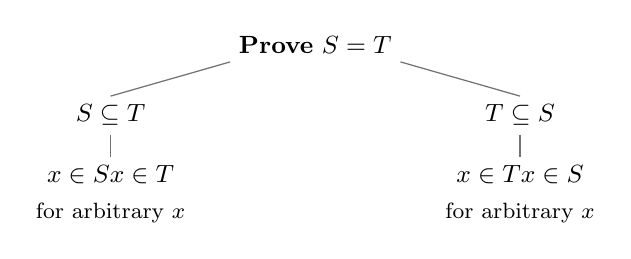
\begin{tikzpicture}[
  x=1cm,y=1cm,font=\small,
  every node/.style={inner sep=3pt,align=center},
  branch/.style={black!55,line width=0.45pt}
]
  \node (goal) at (0,0) {\textbf{Prove} \(S=T\)};
  \node (forward) at (-2.6,-0.9) {\(S\subseteq T\)};
  \node (reverse) at (2.6,-0.9) {\(T\subseteq S\)};
  \node (forward-elements) at (-2.6,-1.9)
    {\(x\in S\implies x\in T\)\\[2pt]
      {\footnotesize for arbitrary \(x\)}};
  \node (reverse-elements) at (2.6,-1.9)
    {\(x\in T\implies x\in S\)\\[2pt]
      {\footnotesize for arbitrary \(x\)}};
  \draw[branch] (goal.south west) -- (forward.north);
  \draw[branch] (goal.south east) -- (reverse.north);
  \draw[branch] (forward.south) -- (forward-elements.north);
  \draw[branch] (reverse.south) -- (reverse-elements.north);
\end{tikzpicture}

  \caption[Proving equality by two inclusions]{A proof tree for set
    equality. Both inclusions are required, and each is proved by
    considering an arbitrary element of the set on the left.}
  \label{fig:linear-algebra-i:set-equality-proof-tree}
\end{figure}
